%%%%%%%%%%%%%%%%%%%%%%%%%%%%%%%%%

\documentclass[12pt]{article} % General page layout

%\usepackage[margin = 1in]{geometry} % For 1 inch margins (includes header)
\usepackage{fullpage} % For 1 inch margins (doesn't include header)
\usepackage{amsmath,textcomp,amssymb} % General math and other packages
\usepackage{fancyhdr} % For page headers and footnotes
\usepackage{graphicx} % For inserting graphs
\usepackage{array} % For matrix
\usepackage{multirow} % Table multiple rows
\usepackage{subfig} % Newer subfigure
\usepackage[T1]{fontenc} % Some math symbols
\usepackage{enumitem} % For custom enumerate labels
\usepackage{listings} % For code appendix

\def\Name{William Ku}  % Your name
\def\ID{wku}  % Your id
\def\Date{02/18/2015} % Due date
\def\Class{16-662 Robot Autonomy} % Class
\def\Proj{2A} % Project #

\pagestyle{fancy}
\headsep = 40pt
\fancyhf{}
\lhead{Project \Proj}
\rhead{\Name\ (\ID)}
\rfoot{\thepage}

%\setcounter{secnumdepth}{0} % Gets rid of the section counter for self definition
\newcolumntype{C}[1]{>{\centering\let\newline\\\arraybackslash\hspace{0pt}}m{#1}}

%%%%%%%%%%%%%%%%%%%%%%%%%%%%%%%%%

\begin{document}

\begin{center}
	\subsection*{\Class\ Project \Proj}
	\paragraph{} \Name\ (Andrew ID:\ \ID)\\\Date
\end{center}


\section{}


\section{Stereo Camera Calibration}
For stereo calibration, five image pairs were selected to perform calibration throughout this section: 72, 2796, 2835, 220, and 3400. We picked {\tt rawleft0001.jpg} and {\tt rawright0001.jpg} for the point correspondences. These correspondences were chosen using MATLAB's built-in function {\tt cpselect}. Figure \ref{corr} shows the 15 point pairs selected from this method. Instead of eight points, 15 points were used as they gave more accurate results using epipolar line match. See Appendix \ref{q2} for the main code.\\

\subsection{Procedure}
To estimate the essential matrix, $ {\bf E_{est}}$, we employed the normalized eight-point algorithm (see Appendix \ref{eightpoint_norm}) to estimate the fundamental matrix, ${\bf F_{est}}$, and obtained the essential matrix using the following relationship:
\begin{equation*}
	\begin{aligned}
		{\bf E_{est}} = {\bf K_{right}}^T{\bf F_{est}}{\bf K_{left}},
	\end{aligned}
\end{equation*}
where ${\bf K_{right}}$ and ${\bf K_{left}}$ are the intrinsic matrices of the right and the left cameras, respectively.
\begin{figure}[b]
	\centering
	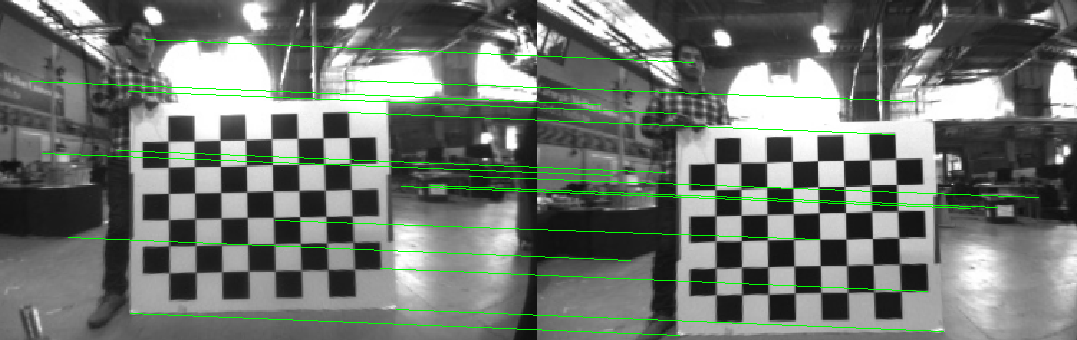
\includegraphics[width=450px]{corr.png}
	\caption{Point Correspondences between {\tt rawleft0001.jpg} and {\tt rawright0001.jpg}.}
	\label{corr}
\end{figure}

\noindent To get the rotation, ${\bf R_{est}}$, and the translation, ${\bf t_{est}}$ estimates, from the left camera to the right camera, we applied the singular value decomposition (SVD) on the estimated essential matrix, ${\bf E_{est}} = {\bf USV}^T$, and constructed ${\bf R_{est}}$ and ${\bf t_{est}}$ using the following formula:
\begin{equation*}
	\begin{aligned}
		W &=
		\left[\begin{array}{ccc}
			0 & -1 & 0\\
			1 & 0 & 0\\
			0 & 0 & 1\\
		\end{array}
		\right],\\
		{\bf R_{est}} &= {\bf UWV}^T\ \ or\ \ {\bf UW}^T{\bf V}^T,\\
		[{\bf t_{est}}]_x &= {\bf VWSV}^T\ \ or\ \ -{\bf VWSV}^T,\\
	\end{aligned}
\end{equation*}
where $[{\bf t_{est}}]_x$ is the skew-symmetric matrix related to ${\bf t_{est}}$ [1]. The resulting ${\bf t_{set}}$ was scaled by the last element for consistency and ease of comparison. The twisted-pair ambiguity outlined in [2] results in four different situations, where only one is physically feasible. This check was done through the triangulation of a point correspondence using the camera matrices. In addition, we enforced the $SO(3)$ criterion, $det({\bf R_{est}}) = 1$, by changing the sign of ${\bf E_{est}}$. Changing of the sign is allowed since ${\bf E_{est}}$ is a projective element and determined up to scale. For the complete code, refer to Appendix \ref{getRt}.\\

\subsection{Evaluation}
${\bf F_{est}}$ and ${\bf F_{gt}}$ were tested against the fundamental matrix relationship, ${\bf x_{right}}^TF{\bf x_{left}} = 0$, and the mean errors for the 15 points are -0.0545 and 1.7949, respectively.\\
The epipoles, ${\bf e_{est}} = [-2202.9, 91.1, 1]^T$ and ${\bf e_{gt}} = [-15271, 151, 1]^T$, of ${\bf F_{est}}$ and ${\bf F_{gt}}$ were also calculated (see Appendix \ref{epipole}).\\
\noindent Using MATLAB's built-in function, {\tt estimateCameraParameters}, the ground truth parameters (${\bf F_{gt}}$, ${\bf E_{gt}}$) were generated for stereo calibration. We compared the fundamental matrices, ${\bf F_{est}}$ and ${\bf F_{gt}}$, by plotting the epipolar lines on the right image given a click point on the left image. Figure \ref{epi} shows the clicked points and the corresponding epipolar lines using ${\bf F_{est}}$ on images {\tt rawleft1796.jpg} and {\tt rawright1796.jpg}. The epipolar lines estimates are quite robust as the they mostly pass through the interest points. Figure \ref{epigt} shows the same image pair using ${\bf F_{gt}}$. With undetermined reasons, the ground truth epipolar lines underperformed on all of the clicks, with epipolar line estimates offsetting the clicked points towards the top. The epipolar line match was performed on randomly selected images and the results were consistent throughout.\\

\begin{figure}[h!]
	\centering
	\subfloat[${\bf F_{est}}$]{%
		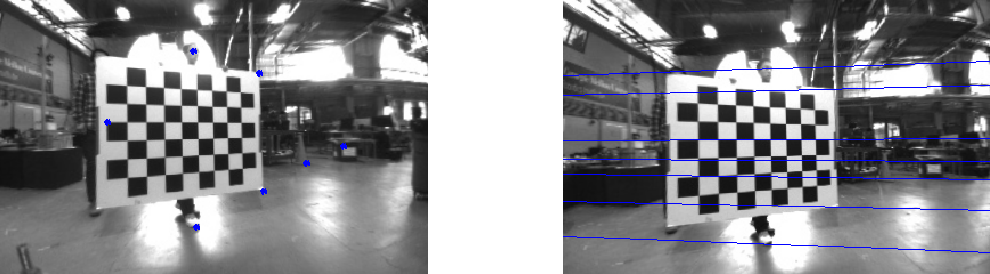
\includegraphics[width=450px]{epipolar2796.png}
		\label{epi}
	}

	\subfloat[${\bf F_{gt}}$]{%
		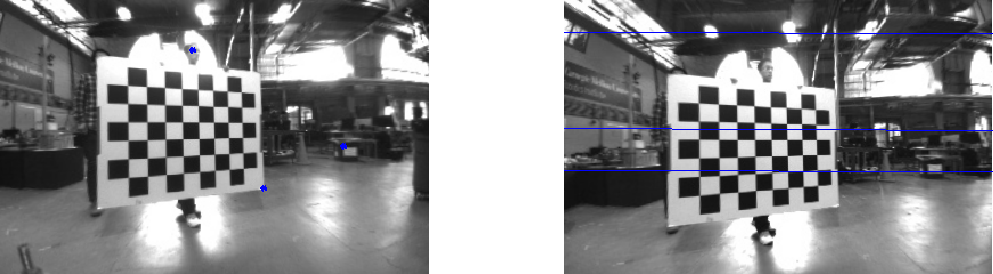
\includegraphics[width=450px]{epipolar2796_gt.png}
		\label{epigt}
	}
	\caption{Clicked Points and Epipolar Lines using Different Fundamental Matrices.}
\end{figure}

\noindent Additionally, ${\bf R_{est}}$ and ${\bf t_{est}}$ were compared to ${\bf R_{gt}}$ and ${\bf t_{gt}}$ calculated from ${\bf E_{gt}}$ using the same decomposition method in Appendix \ref{getRt}:
\begin{equation*}
	\begin{aligned}
		{\bf R_{est}} &= 
		\left[\begin{array}{ccc}
			0.9999 & 0.0101 & 0.0043\\
			-0.0101 & 0.9999 & 0.0079\\
			-0.0042 & -0.0079 & 1.0000\\
		\end{array}\right],\ \ 
		{\bf t_{est}} = 
		\left[\begin{array}{c}
			-14.2947\\ -0.1354\\ 1.0000\\
		\end{array}\right],\\
		{\bf R_{gt}} &= 
		\left[\begin{array}{ccc}
			0.9999 & -0.0040 & -0.0097\\
			0.0040 & 1.0000 & -0.0017\\
			0.0097 & 0.0016 & 1.0000\\
		\end{array}\right],\ \ 
		{\bf t_{gt}} = 
		\left[\begin{array}{c}
			-92.6343\\ 0.1190\\ 1.0000\\
		\end{array}\right].
	\end{aligned}
\end{equation*}
It can be shown that both rotation matrices follow a "${\bf I}$ + skew-symmetric matrix" format, expected from the skew-symmetry (except on the diagonal) of general rotation matrices.\\

\subsection{Conclusion}
Overall, ${\bf F_{est}}$ and ${\bf E_{est}}$ are good enough for our purpose. Without having the actual ${\bf R}$ and ${\bf t}$ from the camera set, we did our best efforts to obtain reasonable estimates for the fundamental matrix and the essential matrix. Tests, such as the fundamental matrix relationship, the epipolar line match, and the $SO(3)$ determinant constraint, helped us verify the integrity of our estimates.

\newpage


\section*{References}
[1] http://en.wikipedia.org/wiki/Essential\_matrix\\[12pt]
[2] Richard Hartley and Andrew Zisserman (2003). Multiple View Geometry in computer vision. Cambridge University Press.

\newpage


\section*{Appendix}
\appendix

\section{Single Camera Calibration}
\label{q1}
\lstinputlisting [language=matlab]{project2a_q1.m}

\section{Camera Calibration Function}
\label{camcalib}
\lstinputlisting [language=matlab]{camcalib.m}

\section{Stereo Camera Calibration}
\label{q2}
\lstinputlisting [language=matlab]{project2a_q2.m}

\section{Normalized Eight-Point Algorithm}
\label{eightpoint_norm}
\lstinputlisting [language=matlab]{eightpoint_norm.m}

\section{Rotation and Translation Estimation}
\label{getRt}
\lstinputlisting [language=matlab]{getRt.m}

\section{Epipole Calculation}
\label{epipole}
\lstinputlisting [language=matlab]{epipole.m}





\end{document}

%%%%%%%%%%%%%%%%%%%%%%%%%%%%%%%%%
% Elements 

\begin{comment}

% Equations
\begin{equation*}
	\begin{aligned}
		H &=
		\left[\begin{array}{c}
			X\\ Y\\ Z\\ 1
		\end{array}\right]
	\end{aligned}
\end{equation*}

% Figure/Subfitures
\begin{figure}[h!]
	\centering
	\includegraphics[width=350px]{xxx.jpg}
	\caption{caption}
	\label{label}
\end{figure}

\begin{figure}[h!]
	\centering
	\subfloat[subcaption1]{%
		\includegraphics[height=150px]{xxx.jpg}
	}
	\subfloat[subcaption2]{%
		\includegraphics[height=150px]{yyy.jpg}
	}
	% An empty line here makes a second row
	\subfloat[subcaption3]{%
		\includegraphics[height=150px]{zzz.jpg}
	}
	\caption{caption}
	\label{label}
\end{figure}

% Tables/subtables
\begin{table}
	\centering
	\subfloat[subcaption1]{
		\begin{tabular}{ | c | c | c | c | }
			\hline
			\  & \multicolumn{3}{ |c| }{Out} \\ \hline
			\multirow{3}{*}{Truths} & X & 0 & 1 \\ \cline{2-4}
			& 0 & 71.75\% & 3.52\% \\ \cline{2-4}
			& 1 & 3.23\% & 21.50\% \\ \hline
		\end{tabular}
	}\hspace{50px}
	\subfloat[subcaption2]{
		\begin{tabular}{ | c | c | c | c | }
			\hline
			\  & \multicolumn{3}{ |c| }{Out} \\ \hline
			\multirow{3}{*}{Truths} & X & 0 & 1 \\ \cline{2-4}
			& 0 & 45.76\% & 21.61\% \\ \cline{2-4}
			& 1 & 5.83\% & 26.8\% \\ \hline
		\end{tabular}
	}
	% An empty line here makes a second row
	\subfloat[subcaption]{
		\begin{tabular}{ | c | c | c | c | }
			\hline
			\  & \multicolumn{3}{ |c| }{Out} \\ \hline
			\multirow{3}{*}{Truths} & X & 0 & 1 \\ \cline{2-4}
			& 0 & 71.43\% & 3.83\% \\ \cline{2-4}
			& 1 & 13.45\% & 11.28\% \\ \hline
		\end{tabular}	}\hspace{50px}
	\subfloat[subcaption]{
		\begin{tabular}{ | c | c | c | c | }
			\hline
			\  & \multicolumn{3}{ |c| }{Out} \\ \hline
			\multirow{3}{*}{Truths} & X & 0 & 1 \\ \cline{2-4}
			& 0 & 52.37\% & 14.99\% \\ \cline{2-4}
			& 1 & 14.88\% & 17.76\% \\ \hline
		\end{tabular}
	}
	\caption{table caption}
\end{table}

% Lists
\begin{enumerate}
	\item item1
	\item item2
	\item item3
\end{enumerate}

% Vertical space
\vspace{20px}

\end{comment}
